
\begin{align}
    P\brak{\frac{1}{4} < X < 1} &= F\brak{1^{-}}-F\brak{\frac{1}{4}} \\
    &= \frac{3}{4} - \brak{\frac{1}{4}}^{2}\\
    &= \frac{11}{16}
\end{align}
\begin{figure}[!ht]
\centering
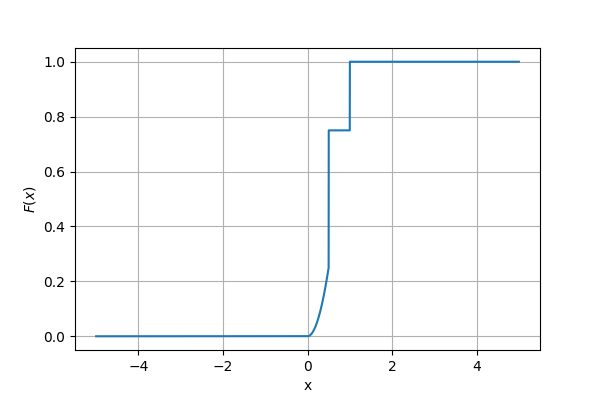
\includegraphics[width=\columnwidth]{solutions/ma/2016/30/figs/Assignment4_CDF.png}
\caption{The CDF of X}
\label{cdf}
\end{figure}


